Before deeper concepts, algorithms and application of undirected graphical models are illustrated, some basics of those models need to be explained. For instance the formal definition of undirected graphs as well as their parameterization.

\subsection{Definition}

TODO: Undirected graphical model = markov network = markov random field \cite{kindermann1980markov} \\
TODO: Markov property (pairwise, local, global) \\
TODO: can be cyclic \\
TODO: cannot represent induced dependency \\
TODO: when the joint probability is strictly positive than it is a Gibbs random field cause it can be represented by the Gibbs measure

As other graphical models like the Bayesian network the undirected graphical network consists of a set of nodes $V$ (also called vertices) and a set of edges between the nodes $E$, which is a set of tuples of exactly two edges. The key difference to a Bayesian network is that those edges are not directed, in the meaning that there is no Direction in the dependency between the nodes, as described in \cite{koller2009probabilistic}.

Undirected Graphs are also called Markov network or Markov random field, when used in a context of probabilistic models. In such case the nodes of the graph are random variables and the edges represent the probabilistic interaction between those variables.

Figure \ref{fig:basic} shows a simple example of a undirected graphical model (markov network) with a set of four random variables $V=\{A,B,C,D\}$ and four probabilistic interactions (edges): $E=\{(A,B),(B,C),(A,C),(C,D)\}$. Thus for example, the nodes could be humans and the edges a probabilistic presentation of how like it is, that two persons are relatives.

\begin{figure}[htpb]
  \centering
  	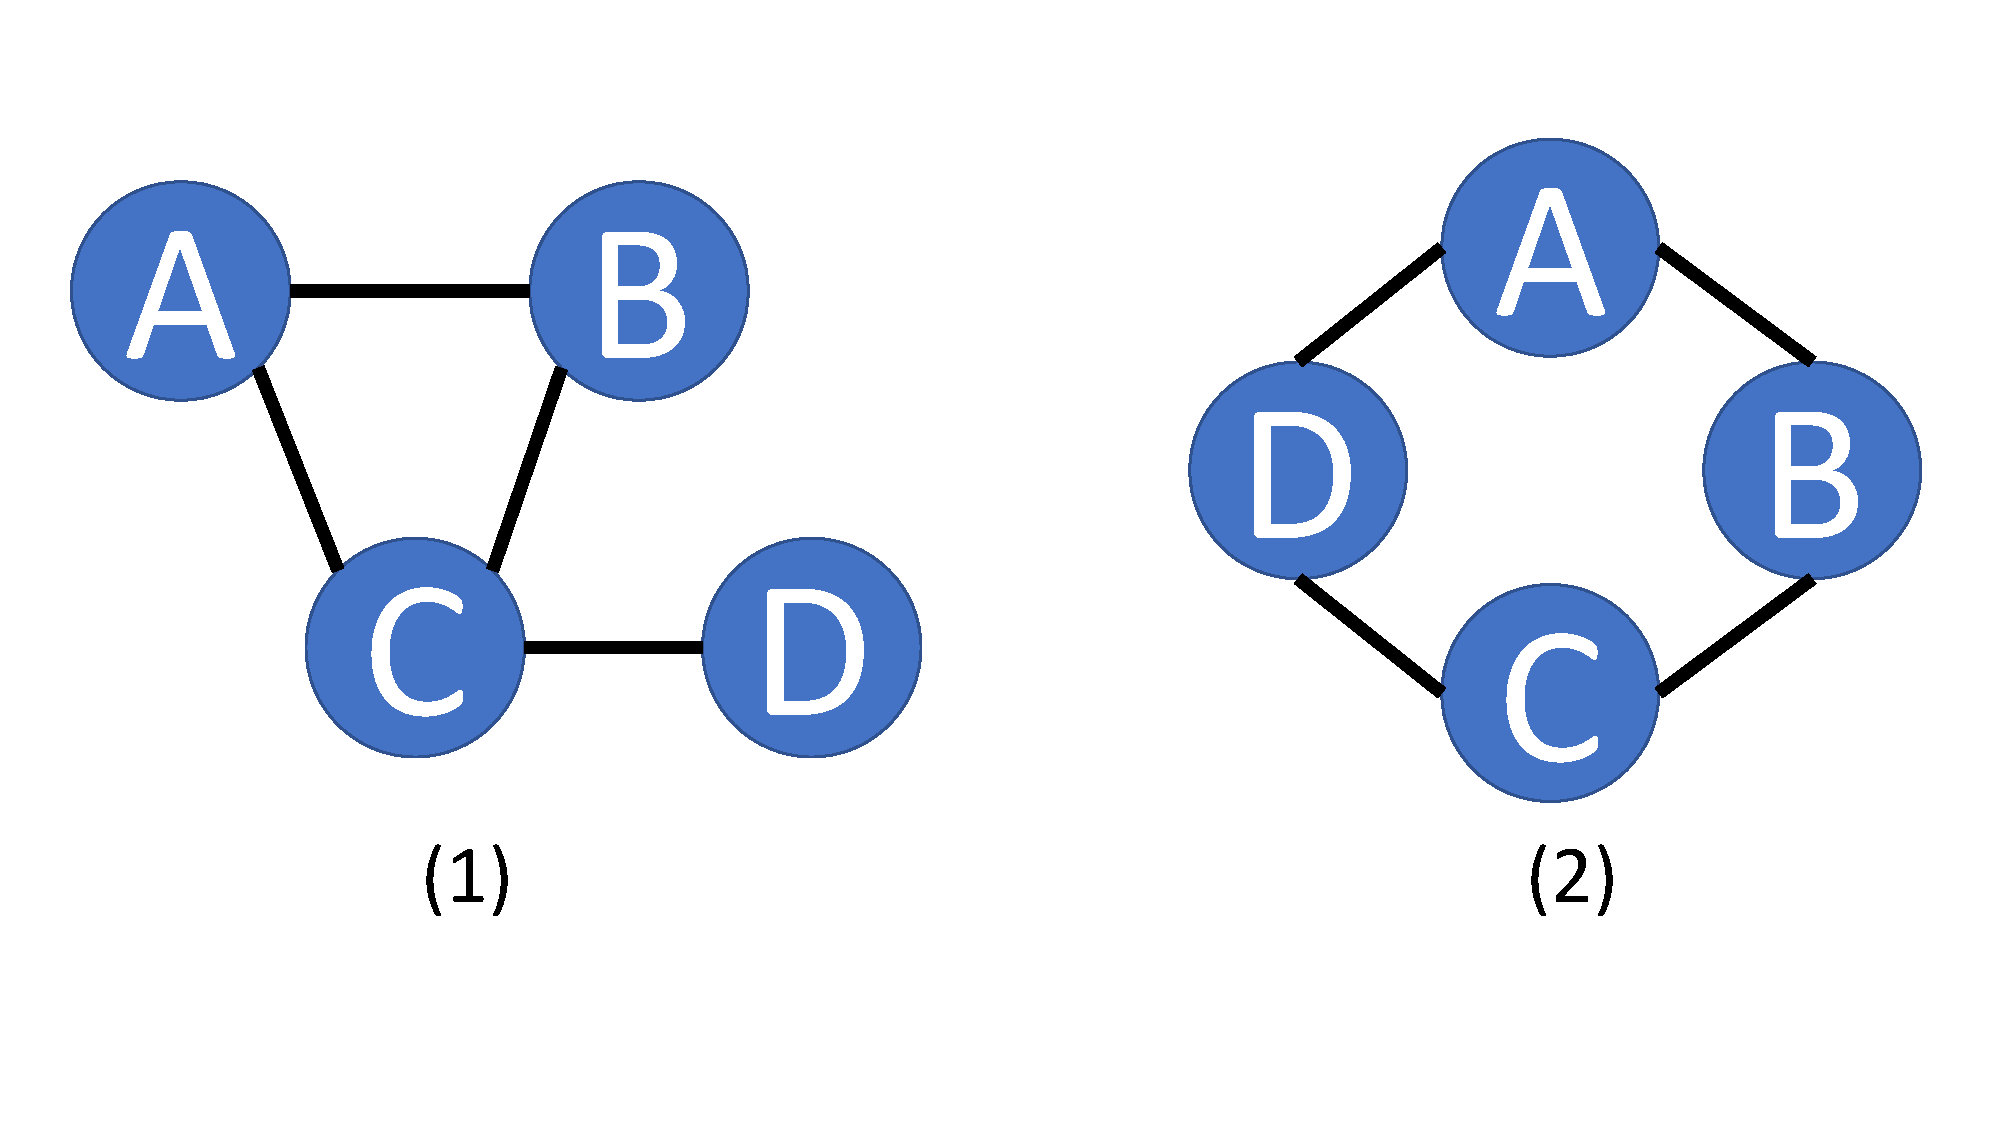
\includegraphics[scale=0.3]{img/basic.pdf} 
  \caption{Simple Undirected Graphical Model}
  \label{fig:basic}
\end{figure}

\subsection{Parameterization}

TODO: clique \\
TODO clique factorization

In order to parameterize the edges between the nodes (means the relation between the random variables) functions, called factors, are defined. 


TODO: factors - unnormalized/normalized


TODO: How does the method work? What are the appealing properties?